
%% bare_conf.tex
%% V1.3
%% 2007/01/11
%% by Michael Shell
%% See:
%% http://www.michaelshell.org/
%% for current contact information.
%%
%% This is a skeleton file demonstrating the use of IEEEtran.cls
%% (requires IEEEtran.cls version 1.7 or later) with an IEEE conference paper.
%%
%% Support sites:
%% http://www.michaelshell.org/tex/ieeetran/
%% http://www.ctan.org/tex-archive/macros/latex/contrib/IEEEtran/
%% and
%% http://www.ieee.org/

%%*************************************************************************
%% Legal Notice:
%% This code is offered as-is without any warranty either expressed or
%% implied; without even the implied warranty of MERCHANTABILITY or
%% FITNESS FOR A PARTICULAR PURPOSE! 
%% User assumes all risk.
%% In no event shall IEEE or any contributor to this code be liable for
%% any damages or losses, including, but not limited to, incidental,
%% consequential, or any other damages, resulting from the use or misuse
%% of any information contained here.
%%
%% All comments are the opinions of their respective authors and are not
%% necessarily endorsed by the IEEE.
%%
%% This work is distributed under the LaTeX Project Public License (LPPL)
%% ( http://www.latex-project.org/ ) version 1.3, and may be freely used,
%% distributed and modified. A copy of the LPPL, version 1.3, is included
%% in the base LaTeX documentation of all distributions of LaTeX released
%% 2003/12/01 or later.
%% Retain all contribution notices and credits.
%% ** Modified files should be clearly indicated as such, including  **
%% ** renaming them and changing author support contact information. **
%%
%% File list of work: IEEEtran.cls, IEEEtran_HOWTO.pdf, bare_adv.tex,
%%                    bare_conf.tex, bare_jrnl.tex, bare_jrnl_compsoc.tex
%%*************************************************************************

% *** Authors should verify (and, if needed, correct) their LaTeX system  ***
% *** with the testflow diagnostic prior to trusting their LaTeX platform ***
% *** with production work. IEEE's font choices can trigger bugs that do  ***
% *** not appear when using other class files.                            ***
% The testflow support page is at:
% http://www.michaelshell.org/tex/testflow/



% Note that the a4paper option is mainly intended so that authors in
% countries using A4 can easily print to A4 and see how their papers will
% look in print - the typesetting of the document will not typically be
% affected with changes in paper size (but the bottom and side margins will).
% Use the testflow package mentioned above to verify correct handling of
% both paper sizes by the user's LaTeX system.
%
% Also note that the "draftcls" or "draftclsnofoot", not "draft", option
% should be used if it is desired that the figures are to be displayed in
% draft mode.
%
\documentclass[conference]{IEEEtran}
% Add the compsoc option for Computer Society conferences.
%
% If IEEEtran.cls has not been installed into the LaTeX system files,
% manually specify the path to it like:
% \documentclass[conference]{../sty/IEEEtran}





% Some very useful LaTeX packages include:
% (uncomment the ones you want to load)


% *** MISC UTILITY PACKAGES ***
%
%\usepackage{ifpdf}
% Heiko Oberdiek's ifpdf.sty is very useful if you need conditional
% compilation based on whether the output is pdf or dvi.
% usage:
% \ifpdf
%   % pdf code
% \else
%   % dvi code
% \fi
% The latest version of ifpdf.sty can be obtained from:
% http://www.ctan.org/tex-archive/macros/latex/contrib/oberdiek/
% Also, note that IEEEtran.cls V1.7 and later provides a builtin
% \ifCLASSINFOpdf conditional that works the same way.
% When switching from latex to pdflatex and vice-versa, the compiler may
% have to be run twice to clear warning/error messages.






% *** CITATION PACKAGES ***
%
%\usepackage{cite}
% cite.sty was written by Donald Arseneau
% V1.6 and later of IEEEtran pre-defines the format of the cite.sty package
% \cite{} output to follow that of IEEE. Loading the cite package will
% result in citation numbers being automatically sorted and properly
% "compressed/ranged". e.g., [1], [9], [2], [7], [5], [6] without using
% cite.sty will become [1], [2], [5]--[7], [9] using cite.sty. cite.sty's
% \cite will automatically add leading space, if needed. Use cite.sty's
% noadjust option (cite.sty V3.8 and later) if you want to turn this off.
% cite.sty is already installed on most LaTeX systems. Be sure and use
% version 4.0 (2003-05-27) and later if using hyperref.sty. cite.sty does
% not currently provide for hyperlinked citations.
% The latest version can be obtained at:
% http://www.ctan.org/tex-archive/macros/latex/contrib/cite/
% The documentation is contained in the cite.sty file itself.






% *** GRAPHICS RELATED PACKAGES ***
%
\ifCLASSINFOpdf
  \usepackage[pdftex]{graphicx}
  % declare the path(s) where your graphic files are
  \graphicspath{{figures}{figures/preliminary}}
  % and their extensions so you won't have to specify these with
  % every instance of \includegraphics
  \DeclareGraphicsExtensions{.pdf,.jpeg,.png}
\else
  % or other class option (dvipsone, dvipdf, if not using dvips). graphicx
  % will default to the driver specified in the system graphics.cfg if no
  % driver is specified.
  % \usepackage[dvips]{graphicx}
  % declare the path(s) where your graphic files are
  % \graphicspath{{../eps/}}
  % and their extensions so you won't have to specify these with
  % every instance of \includegraphics
  % \DeclareGraphicsExtensions{.eps}
\fi
% graphicx was written by David Carlisle and Sebastian Rahtz. It is
% required if you want graphics, photos, etc. graphicx.sty is already
% installed on most LaTeX systems. The latest version and documentation can
% be obtained at: 
% http://www.ctan.org/tex-archive/macros/latex/required/graphics/
% Another good source of documentation is "Using Imported Graphics in
% LaTeX2e" by Keith Reckdahl which can be found as epslatex.ps or
% epslatex.pdf at: http://www.ctan.org/tex-archive/info/
%
% latex, and pdflatex in dvi mode, support graphics in encapsulated
% postscript (.eps) format. pdflatex in pdf mode supports graphics
% in .pdf, .jpeg, .png and .mps (metapost) formats. Users should ensure
% that all non-photo figures use a vector format (.eps, .pdf, .mps) and
% not a bitmapped formats (.jpeg, .png). IEEE frowns on bitmapped formats
% which can result in "jaggedy"/blurry rendering of lines and letters as
% well as large increases in file sizes.
%
% You can find documentation about the pdfTeX application at:
% http://www.tug.org/applications/pdftex





% *** MATH PACKAGES ***
%
%\usepackage[cmex10]{amsmath}
% A popular package from the American Mathematical Society that provides
% many useful and powerful commands for dealing with mathematics. If using
% it, be sure to load this package with the cmex10 option to ensure that
% only type 1 fonts will utilized at all point sizes. Without this option,
% it is possible that some math symbols, particularly those within
% footnotes, will be rendered in bitmap form which will result in a
% document that can not be IEEE Xplore compliant!
%
% Also, note that the amsmath package sets \interdisplaylinepenalty to 10000
% thus preventing page breaks from occurring within multiline equations. Use:
%\interdisplaylinepenalty=2500
% after loading amsmath to restore such page breaks as IEEEtran.cls normally
% does. amsmath.sty is already installed on most LaTeX systems. The latest
% version and documentation can be obtained at:
% http://www.ctan.org/tex-archive/macros/latex/required/amslatex/math/





% *** SPECIALIZED LIST PACKAGES ***
%
%\usepackage{algorithmic}
% algorithmic.sty was written by Peter Williams and Rogerio Brito.
% This package provides an algorithmic environment fo describing algorithms.
% You can use the algorithmic environment in-text or within a figure
% environment to provide for a floating algorithm. Do NOT use the algorithm
% floating environment provided by algorithm.sty (by the same authors) or
% algorithm2e.sty (by Christophe Fiorio) as IEEE does not use dedicated
% algorithm float types and packages that provide these will not provide
% correct IEEE style captions. The latest version and documentation of
% algorithmic.sty can be obtained at:
% http://www.ctan.org/tex-archive/macros/latex/contrib/algorithms/
% There is also a support site at:
% http://algorithms.berlios.de/index.html
% Also of interest may be the (relatively newer and more customizable)
% algorithmicx.sty package by Szasz Janos:
% http://www.ctan.org/tex-archive/macros/latex/contrib/algorithmicx/




% *** ALIGNMENT PACKAGES ***
%
%\usepackage{array}
% Frank Mittelbach's and David Carlisle's array.sty patches and improves
% the standard LaTeX2e array and tabular environments to provide better
% appearance and additional user controls. As the default LaTeX2e table
% generation code is lacking to the point of almost being broken with
% respect to the quality of the end results, all users are strongly
% advised to use an enhanced (at the very least that provided by array.sty)
% set of table tools. array.sty is already installed on most systems. The
% latest version and documentation can be obtained at:
% http://www.ctan.org/tex-archive/macros/latex/required/tools/


%\usepackage{mdwmath}
%\usepackage{mdwtab}
% Also highly recommended is Mark Wooding's extremely powerful MDW tools,
% especially mdwmath.sty and mdwtab.sty which are used to format equations
% and tables, respectively. The MDWtools set is already installed on most
% LaTeX systems. The lastest version and documentation is available at:
% http://www.ctan.org/tex-archive/macros/latex/contrib/mdwtools/


% IEEEtran contains the IEEEeqnarray family of commands that can be used to
% generate multiline equations as well as matrices, tables, etc., of high
% quality.


%\usepackage{eqparbox}
% Also of notable interest is Scott Pakin's eqparbox package for creating
% (automatically sized) equal width boxes - aka "natural width parboxes".
% Available at:
% http://www.ctan.org/tex-archive/macros/latex/contrib/eqparbox/





% *** SUBFIGURE PACKAGES ***
%\usepackage[tight,footnotesize]{subfigure}
% subfigure.sty was written by Steven Douglas Cochran. This package makes it
% easy to put subfigures in your figures. e.g., "Figure 1a and 1b". For IEEE
% work, it is a good idea to load it with the tight package option to reduce
% the amount of white space around the subfigures. subfigure.sty is already
% installed on most LaTeX systems. The latest version and documentation can
% be obtained at:
% http://www.ctan.org/tex-archive/obsolete/macros/latex/contrib/subfigure/
% subfigure.sty has been superceeded by subfig.sty.



%\usepackage[caption=false]{caption}
%\usepackage[font=footnotesize]{subfig}
% subfig.sty, also written by Steven Douglas Cochran, is the modern
% replacement for subfigure.sty. However, subfig.sty requires and
% automatically loads Axel Sommerfeldt's caption.sty which will override
% IEEEtran.cls handling of captions and this will result in nonIEEE style
% figure/table captions. To prevent this problem, be sure and preload
% caption.sty with its "caption=false" package option. This is will preserve
% IEEEtran.cls handing of captions. Version 1.3 (2005/06/28) and later 
% (recommended due to many improvements over 1.2) of subfig.sty supports
% the caption=false option directly:
%\usepackage[caption=false,font=footnotesize]{subfig}
%
% The latest version and documentation can be obtained at:
% http://www.ctan.org/tex-archive/macros/latex/contrib/subfig/
% The latest version and documentation of caption.sty can be obtained at:
% http://www.ctan.org/tex-archive/macros/latex/contrib/caption/




% *** FLOAT PACKAGES ***
%
%\usepackage{fixltx2e}
% fixltx2e, the successor to the earlier fix2col.sty, was written by
% Frank Mittelbach and David Carlisle. This package corrects a few problems
% in the LaTeX2e kernel, the most notable of which is that in current
% LaTeX2e releases, the ordering of single and double column floats is not
% guaranteed to be preserved. Thus, an unpatched LaTeX2e can allow a
% single column figure to be placed prior to an earlier double column
% figure. The latest version and documentation can be found at:
% http://www.ctan.org/tex-archive/macros/latex/base/



%\usepackage{stfloats}
% stfloats.sty was written by Sigitas Tolusis. This package gives LaTeX2e
% the ability to do double column floats at the bottom of the page as well
% as the top. (e.g., "\begin{figure*}[!b]" is not normally possible in
% LaTeX2e). It also provides a command:
%\fnbelowfloat
% to enable the placement of footnotes below bottom floats (the standard
% LaTeX2e kernel puts them above bottom floats). This is an invasive package
% which rewrites many portions of the LaTeX2e float routines. It may not work
% with other packages that modify the LaTeX2e float routines. The latest
% version and documentation can be obtained at:
% http://www.ctan.org/tex-archive/macros/latex/contrib/sttools/
% Documentation is contained in the stfloats.sty comments as well as in the
% presfull.pdf file. Do not use the stfloats baselinefloat ability as IEEE
% does not allow \baselineskip to stretch. Authors submitting work to the
% IEEE should note that IEEE rarely uses double column equations and
% that authors should try to avoid such use. Do not be tempted to use the
% cuted.sty or midfloat.sty packages (also by Sigitas Tolusis) as IEEE does
% not format its papers in such ways.





% *** PDF, URL AND HYPERLINK PACKAGES ***
%
\usepackage{url}
% url.sty was written by Donald Arseneau. It provides better support for
% handling and breaking URLs. url.sty is already installed on most LaTeX
% systems. The latest version can be obtained at:
% http://www.ctan.org/tex-archive/macros/latex/contrib/misc/
% Read the url.sty source comments for usage information. Basically,
% \url{my_url_here}.



% *** Do not adjust lengths that control margins, column widths, etc. ***
% *** Do not use packages that alter fonts (such as pslatex).         ***
% There should be no need to do such things with IEEEtran.cls V1.6 and later.
% (Unless specifically asked to do so by the journal or conference you plan
% to submit to, of course. )

\usepackage{tabularx}
\usepackage{booktabs}

% correct bad hyphenation here
\hyphenation{op-tical net-works semi-conduc-tor}


\begin{document}
	
\newcommand{\note}[1]{**{#1}}
\newcommand{\boldnote}[1]{\textbf{**{#1}}}

\newcommand{\rqtutorial}{RQ1: Do end-user programmers even complete tutorials?}
\newcommand{\rqengagement}{RQ2: What effect does completing tutorials have on end user programmers' engagement?}
\newcommand{\rqlearning}{RQ3: What effect does completing tutorials have on end-user programmers' learning?}

%
% paper title
% can use linebreaks \\ within to get better formatting as desired
\title{Effects of Tutorials on End-User Programmer Feature Usage and Engagement in TouchDevelop** (temporary title)}


% author names and affiliations
% use a multiple column layout for up to three different
% affiliations
\author{\IEEEauthorblockN{Sergii and Irwin and Austin}
\IEEEauthorblockA{Department of Electrical Engineering \& Computer Science\\
Oregon State University\\
Corvallis, Oregon, 97330
Email: {sergii,kwan}@eecs.oregonstate.edu}
}

% conference papers do not typically use \thanks and this command
% is locked out in conference mode. If really needed, such as for
% the acknowledgment of grants, issue a \IEEEoverridecommandlockouts
% after \documentclass

% for over three affiliations, or if they all won't fit within the width
% of the page, use this alternative format:
% 
%\author{\IEEEauthorblockN{Michael Shell\IEEEauthorrefmark{1},
%Homer Simpson\IEEEauthorrefmark{2},
%James Kirk\IEEEauthorrefmark{3}, 
%Montgomery Scott\IEEEauthorrefmark{3} and
%Eldon Tyrell\IEEEauthorrefmark{4}}
%\IEEEauthorblockA{\IEEEauthorrefmark{1}School of Electrical and Computer Engineering\\
%Georgia Institute of Technology,
%Atlanta, Georgia 30332--0250\\ Email: see http://www.michaelshell.org/contact.html}
%\IEEEauthorblockA{\IEEEauthorrefmark{2}Twentieth Century Fox, Springfield, USA\\
%Email: homer@thesimpsons.com}
%\IEEEauthorblockA{\IEEEauthorrefmark{3}Starfleet Academy, San Francisco, California 96678-2391\\
%Telephone: (800) 555--1212, Fax: (888) 555--1212}
%\IEEEauthorblockA{\IEEEauthorrefmark{4}Tyrell Inc., 123 Replicant Street, Los Angeles, California 90210--4321}}




% use for special paper notices
%\IEEEspecialpapernotice{(Invited Paper)}




% make the title area
\maketitle


\begin{abstract}
%\boldmath
As programming becomes an increasingly valuable skillset in the modern world, there are many methods available to learn how to program. One method gaining popularity with more complex web apps is that of the interactive tutorial. We examine users� published scripts on the TouchDevelop platform and compare interactive tutorials to traditional, copy-and-paste tutorial methods in terms of user outcomes.
To accomplish this, we build a tool to facilitate large-scale data capture and analysis of TouchDevelop users and scripts. This tool is also capable of facilitating a much broader scope of research questions concerning the TouchDevelop population.
\end{abstract}
% IEEEtran.cls defaults to using nonbold math in the Abstract.
% This preserves the distinction between vectors and scalars. However,
% if the conference you are submitting to favors bold math in the abstract,
% then you can use LaTeX's standard command \boldmath at the very start
% of the abstract to achieve this. Many IEEE journals/conferences frown on
% math in the abstract anyway.

% no keywords




% For peer review papers, you can put extra information on the cover
% page as needed:
% \ifCLASSOPTIONpeerreview
% \begin{center} \bfseries EDICS Category: 3-BBND \end{center}
% \fi
%
% For peerreview papers, this IEEEtran command inserts a page break and
% creates the second title. It will be ignored for other modes.
\IEEEpeerreviewmaketitle


%!TEX root = touchdevelop_tutorials.tex
\section{Introduction}
% no \IEEEPARstart

Programming has, over the last 60 years, become an increasingly popular discipline, both as a primary profession and as a hobby or additional job skill. Traditionally most self-taught programmers learn from a book or a website that intersperses writing with code snippets that can be copied and pasted into a source code editor.
However, in recent years the advent of rich web apps that are able to respond to the user dynamically have begun to change how programming is taught. The website Codecademy [4], for example, presents all its tutorials via a web app that also functions as an IDE, complete with progress indicators, hints, and tests to make sure the user�s code is correct. The site Code School [5] advertises by saying �Enjoy an education in the comfort of your browser�. Another new source of interactive programming tutorials is TouchDevelop [9]. This platform is intended to teach and enable end-user programmers on touch-based devices such as smartphones or tablets to create their own scripts. As both a new programming paradigm and a new programming language, it necessarily involves a large amount of teaching users new to programming, TouchDevelop, or both.

\begin{itemize}
\item What effect do tutorials have on end-user programmer feature usage?
\item What effect do tutorials have on end-user programmer engagement?
\end{itemize}
%!TEX root = touchdevelop_tutorials.tex
\section{Background}

\subsection{TouchDevelop}

TouchDevelop is an experimental programming platform for end-user programming on touch-screen devices. It is also designed a research tool, meaning that published projects are automatically open sourced, and a wealth of data on users and published scripts is made public (see [3]) on a growing userbase. However, while the JSON-based APIs are very useful for looking at specific scripts or examining scripts one at a time, large-scale relational-database style queries are unavailable in the TouchDevelop API.

As a result, studies of the TouchDevelop population such as Athreya et al. [1] have had to rely on a random sample of scripts, classified by hand. First and most importantly, this greatly limits the size of the sample. Secondly, it introduces personal bias and error into the process - Athreya et al.’s study [1] describes the process of ‘negotiation’ when researchers inevitably disagreed on classification of scripts.

One particular case of this was the category of No Meaningful Functionality scripts in [Balaji’s paper]. This made up a significant portion of the TouchDevelop script base, and included tutorials, among other published scripts that would not be useful to anyone besides the author. However, due undoubtedly to a desire to not waste time, this category of scripts was not detailed further.

Li et al. [2] studied the behavior of users in TouchDevelop. They found that 68.3\% of TouchDevelop users published one or two scripts and then never returned or produced more content. This begs the question: why? This is an especially important question, as TouchDevelop is a novel approach to programming and is intended for end user programmers, many of whom may have had no previous experience programming at all, and thus do not even know basic concepts such as variables and functions.

\subsection{Tutorials and Community Engagement}

\boldnote{Programming languages are difficult to learn, and many resources have been devoted to increasing retention and interest in end-user programming languages.} A new programming language is difficult to learn, especially for an end-user developer. These end-user developers often need to learn on their own, without the support of peers.

Analysis of end-user developer repositories
\cite{athreya2012:touchdevelop,bogart2008:coscripter,sihan2013:touchdevelop,stolee2013:yahoopipes} has shown that reuse between scripts is very low. In addition, user retention is also very low. In what ways can we improve user retention? 

However, little research has been done specifically investigating what effect making training material, such as tutorials, available to end-user programmers has on their engagement and adoption of the platform.

\note{Need argument here that we should understand effects of tutorials on user engagement}
Open-source projects have their own ways of maintaining documentation~\cite{dagenais2010} (cite other papers about the use of documentation for learning APIs, libraries, and programming). However, Carroll and Rosson~\cite{carroll_paradox_1987} identified that tutorials were also not appropriate for ``active users'', who were more concerned about completing tasks than learning.

\boldnote{The TouchDevelop environment had interactive tutorials and non-interactive tutorials and they were different in a few ways}
The TouchDevelop environment has interactive tutorials and non-interactive tutorials. From a learning standpoint, interactive tutorials seem superior; for example ... Stencils (Kelleher), LemonAid (Andy Ko). There are reasons to consider non-interactive tutorials. For instance, a study of \emph{opportunistic programmers} identified them as quickly copying and pasting snippets from tutorials to learn new skills and approaches, which would not be possible with an interactive tutorial~\cite{brandt2009:opportunistic}.

\note{Strangely enough, the tutorials don't have any accompanying plain English language text with them. Some of them have documentation, some do not.}


There are two types of TouchDevelop tutorials available: interactive and non-interactive. Interactive tutorials engage the user into tutorial completion more actively than non-interactive tutorials by providing frequent direct suggestions on what user is supposed to do next. On the other hand, non-interactive tutorials provide tutorial instructions and source code snippets without guiding the user directly.

%!TEX root = touchdevelop_tutorials.tex
\section{Method}

To conduct our study, we used the public TouchDevelop API to extract 35000 scripts which we stored in a MySQL database.

\subsection{Analysis}

We used SQL queries and statistical methods to examine our data.

As our data tended to be heavily skewed to the left, we used non-parametric statistics, such as Kruskal-Wallis.

\note{Please verify} To identify a script as a tutorial, we... (describe how we identified the initial tutorial script. Was it that we went to the web site and then looked at the site? Or, based on naming? Or something else?)

\note{Sergii please verify} Scripts (**that users create as a result of following a tutorial**???**) are tagged with \texttt{\#doc}, \texttt{\#tutorials}, or \texttt{\#interactiveTutorial} in the case of an interactive tutorial.


We identified that tutorials were tagged with the \#doc hashtag and that there are a total of XX tutorials.

\boldnote{When appropriate, we removed some usernames from our analysis.}
We contacted the TouchDevelop team and learned further that certain author names, including ``TouchDevelop Samples'' and ``TouchDevelop Documentation'', were operated by Microsoft employees; in our author data analysis we remove these from the analysis. \note{Be really specific when we actually do this. we might have to rewrite this statement}

\note{There are some group accounts based on the account name and activity. We cannot be certain, however, we can only guess and this has to be a threat to validity.}

%!TEX root = touchdevelop_tutorials.tex
\section{Results}

Our results are...
%!TEX root = touchdevelop_tutorials.tex

\subsection{\rqtutorial}

% -- Running on Jan 27 db:
% Authors who published one or more scripts	19122
% Authors who did not attempt a tutorial	17740
% Authors attempted or completed a tutorial	1382
% Authors who attempted (but did not complete) a tutorial	578
% Authors who completed exactly one tutorial	708
% Authors who completed two or more tutorials	96

\def\numauthors{19122}%
\def\authorsNoUsedTutorials{17740}%
\def\authorsUsedTutorials{1382}%
\def\authorsZeroTutorials{578}%
\def\authorsOneTutorials{708}%
\def\authorsTwoTutorials{96}%

\def\totalcompletions{\FPeval\result{\authorsOneTutorials+\authorsTwoTutorials}%
\FPround\result{\result}{0}%
\result%
}

In general, TouchDevelop script authors are only somewhat willing to attempt tutorials.
Of the \numauthors{} users who have published at least one script, we observed that only \authorsUsedTutorials{} (7.2\%) attempted a tutorial and only \totalcompletions{} (4.2\%) of all users completed one or more tutorials.


\begin{table}
	\centering
	\begin{tabular}{rr}
		\toprule
		Authors who published one or more scripts & \numauthors{} (100\%)\\
		\midrule
		Authors who did not attempt a tutorial & \authorsNoUsedTutorials{} (92.8\%)\\
		Authors who attempted or completed a tutorial & \authorsUsedTutorials{} (7.2\%)\\
		\midrule
		Authors who attempted (but did not complete) a tutorial & \authorsZeroTutorials{} (3.0\%)\\
		Authors who completed one tutorial & \authorsOneTutorials{} (3.7\%)\\
		Authors who completed more than tutorial & \authorsTwoTutorials{} (0.5\%)\\
		\bottomrule
	\end{tabular}
	\caption{Proportion of TouchDevelop users who complete tutorials. Only 7.2\% of users attempt tutorials and 4.2\% complete one or more tutorials.}
	\label{tab:tutorial_completions}
\end{table}

The following tutorials were the ones that were most frequently completed by our participants.

% Attempts
% scratch pong tutorial	1
% scratch cat tutorial	1
% pixels tutorial	1
% bouncing monster tutorial	4
% Build Your First App M4T3	8
% Diamonds and Rubys	23
% bubble popper tutorial	26
% physics game walkthrough	279
% Bounce (physics)	279
% first steps with drawing	417

% Completions
% Build Your First App M3T4	1
% Dice tutorial	1
% data	1
% doitall browser	2
% amazing script 2	2
% for each	3
% soundboard tutorial	4
% doitall browser 4	9
% Diamonds and Rubys	27
% crazy holiday football demo	34
% accelero-turtle	34
% Build Your First App M3T2	40
% scratch pong tutorial	81
% beatbox tutorial	260
% pixels tutorial	381

\begin{table}
	\centering
	\begin{tabular}{lrr}
		\toprule
		Tutorial & Attempts & Completions\\\midrule
		scratch cat tutorial &	1 & 0 \\
		bouncing monaster tutorial &	4 & 0 \\
		Build Your First App M4T3 &	8 &	0\\
		bubble popper tutorial & 26 & 0 \\
		physics game walkthrough/Bounce (physics) &	279 & 0 \\
		first steps with drawing & 417 & 0 \\
		Build Your First App M3T4 & 0 & 1\\
		Dice tutorial &	0 & 1\\
		data & 0 & 1\\
		doital browser & 0 & 2\\
		amazing script 2 & 0 & 2\\
		for each & 0 & 3\\
		soundboard tutorial & 0 & 4\\
		doitall browser 4 &	0 &	9\\
		Diamonds and Rubys &	23 &	27\\
		crazy holiday football demo &	0 &	34\\
		accelero-turtle &	0 &	34\\
		Build Your First App M3T2 & 0 &	40\\
		scratch pong tutorial &	1 &	81\\
		beatbox tutorial &	0 &	260\\
		pixels tutorial &	1 &	381\\
		\bottomrule
	\end{tabular}
	\caption{Proportion of TouchDevelop users who complete tutorials. Only 7.2\% of users attempt tutorials and 4.2\% complete one or more tutorials.}
	\label{tab:tutorial_completions}
\end{table}

% Some notes about the tutorials:
% first steps with drawing https://www.touchdevelop.com/api/ayyxc is no longer available publically, it can't be accessed.

One severe limitation of this data is that there are very few attempts on tutorials. One reason for this would be because of data collection. Since we could only collect published scripts, authors who attempted tutorials but did not finish them would have to publish them explicitly, which would not be expected if the script is unfinished or not working.

\note{Implication?} Despite this finding, our data still shows that a large number of users have successfully published scripts. This suggests that many TouchDevelop users are either familiar with programming and did not require tutorials or that they learned or were taught TouchDevelop offline (for example, as part of an outreach effort or by friends). There is also the possibility that users generally avoided the official tutorials and used other resources, but non-Microsoft tutorials are rather rare. \note{One way to explore this further is to examine the features of scripts that people who didn't use tutorials had. If they are filled with advanced constructs then we can assume that they have some prior knowledge}


\note{Data limitation: it seems that physics game walkthrough and Bounce (physics) have code fragment overlaps, as they co-occur in the database. For this reason we should consider them to be a single data point, we cannot read into it further.}






%!TEX root = touchdevelop_tutorials.tex

\subsection{\rqengagement}

We compared the average usage statistics of authors who completed zero, one, and more than one tutorial in TouchDevelop.


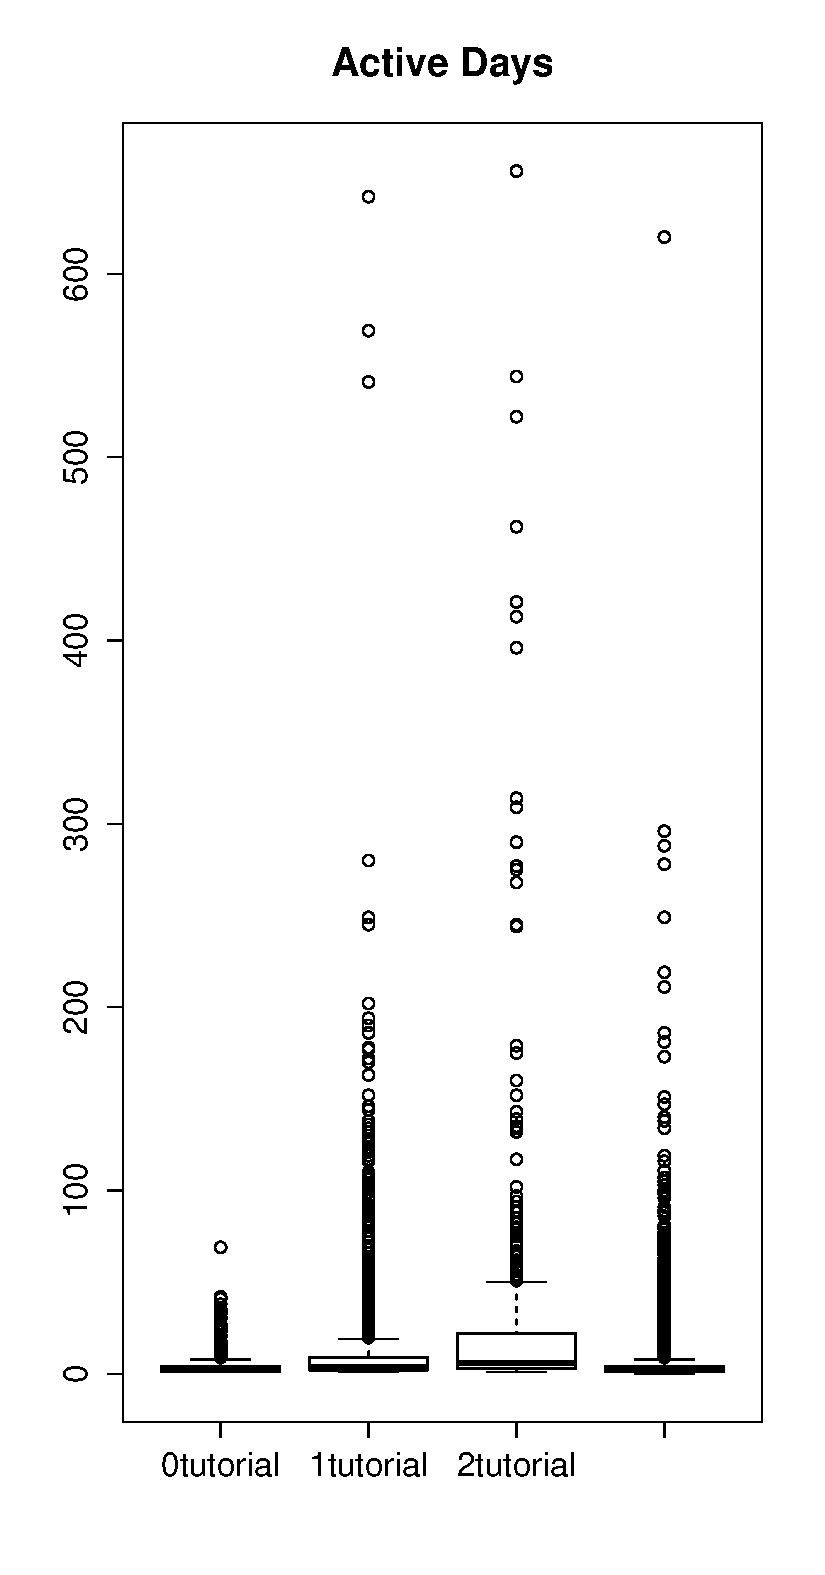
\includegraphics[width=\columnwidth]{figures/preliminary/activedays_boxplot}
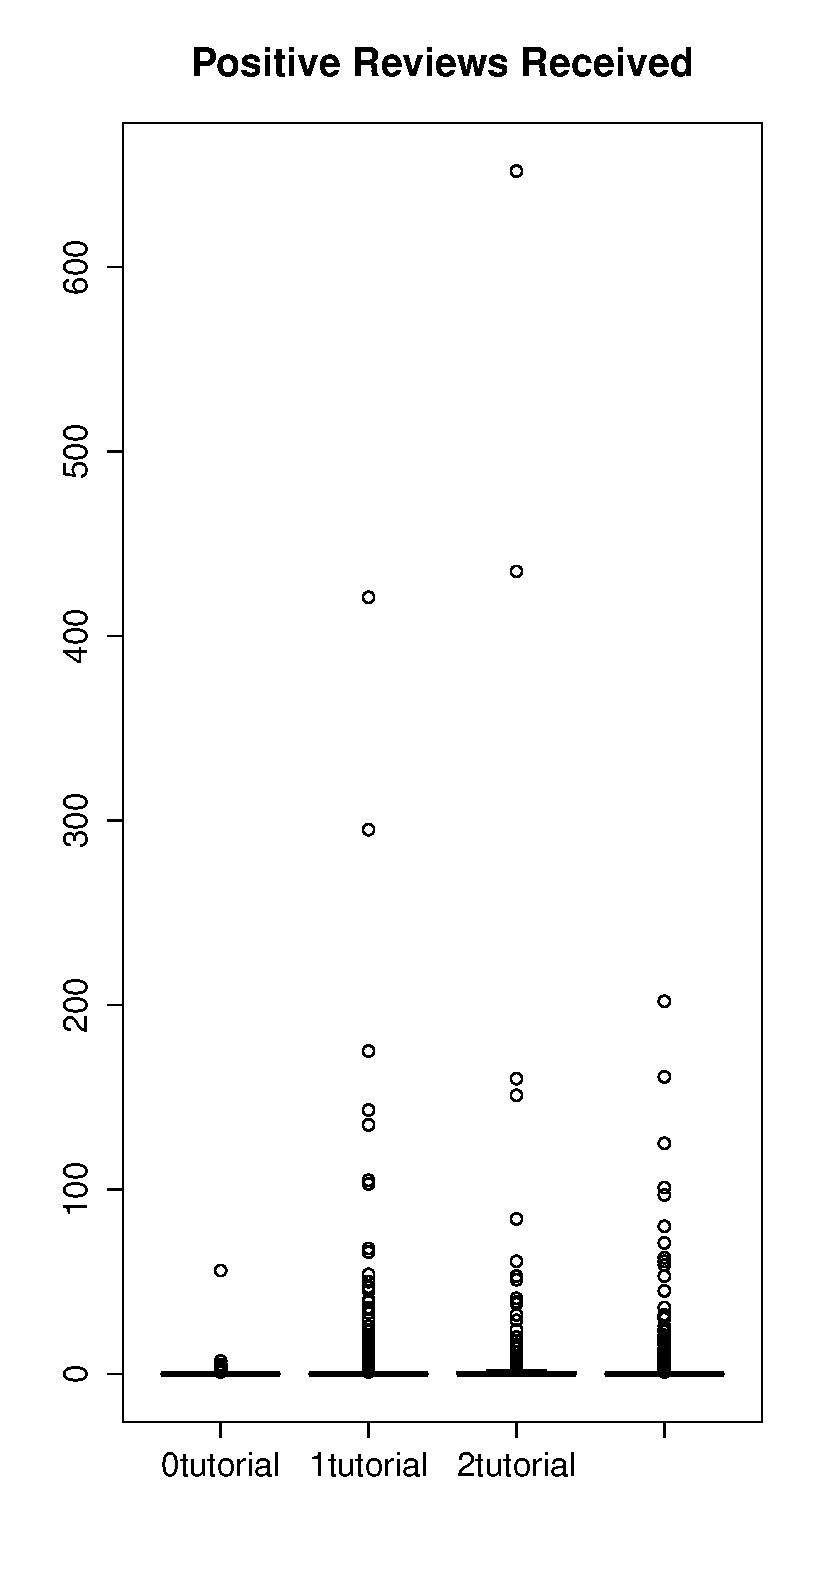
\includegraphics[width=\columnwidth]{figures/preliminary/positivereviews_boxplot}
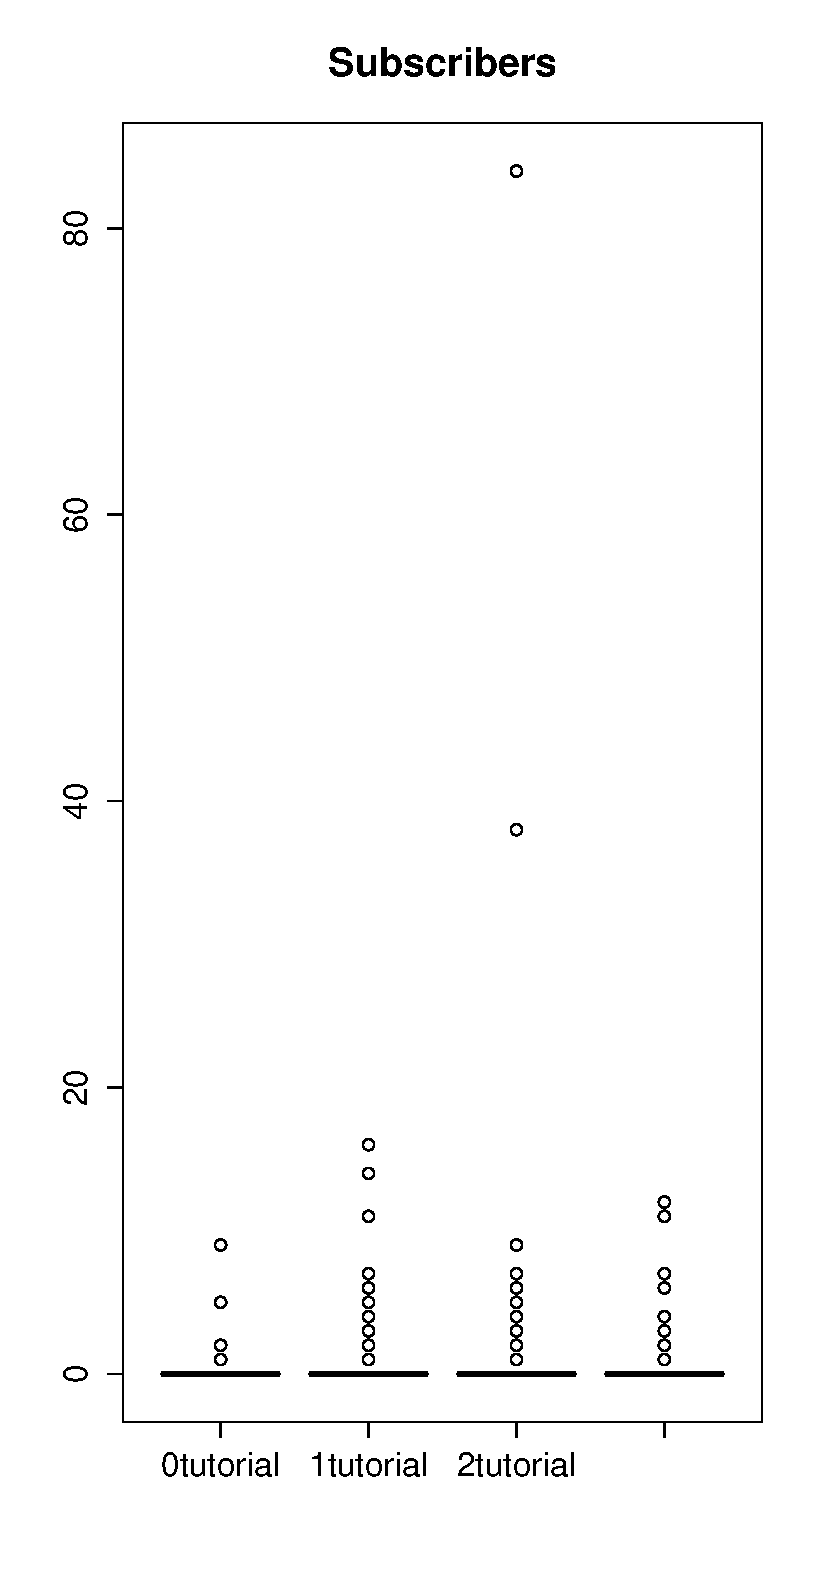
\includegraphics[width=\columnwidth]{figures/preliminary/subscribers_boxplot}
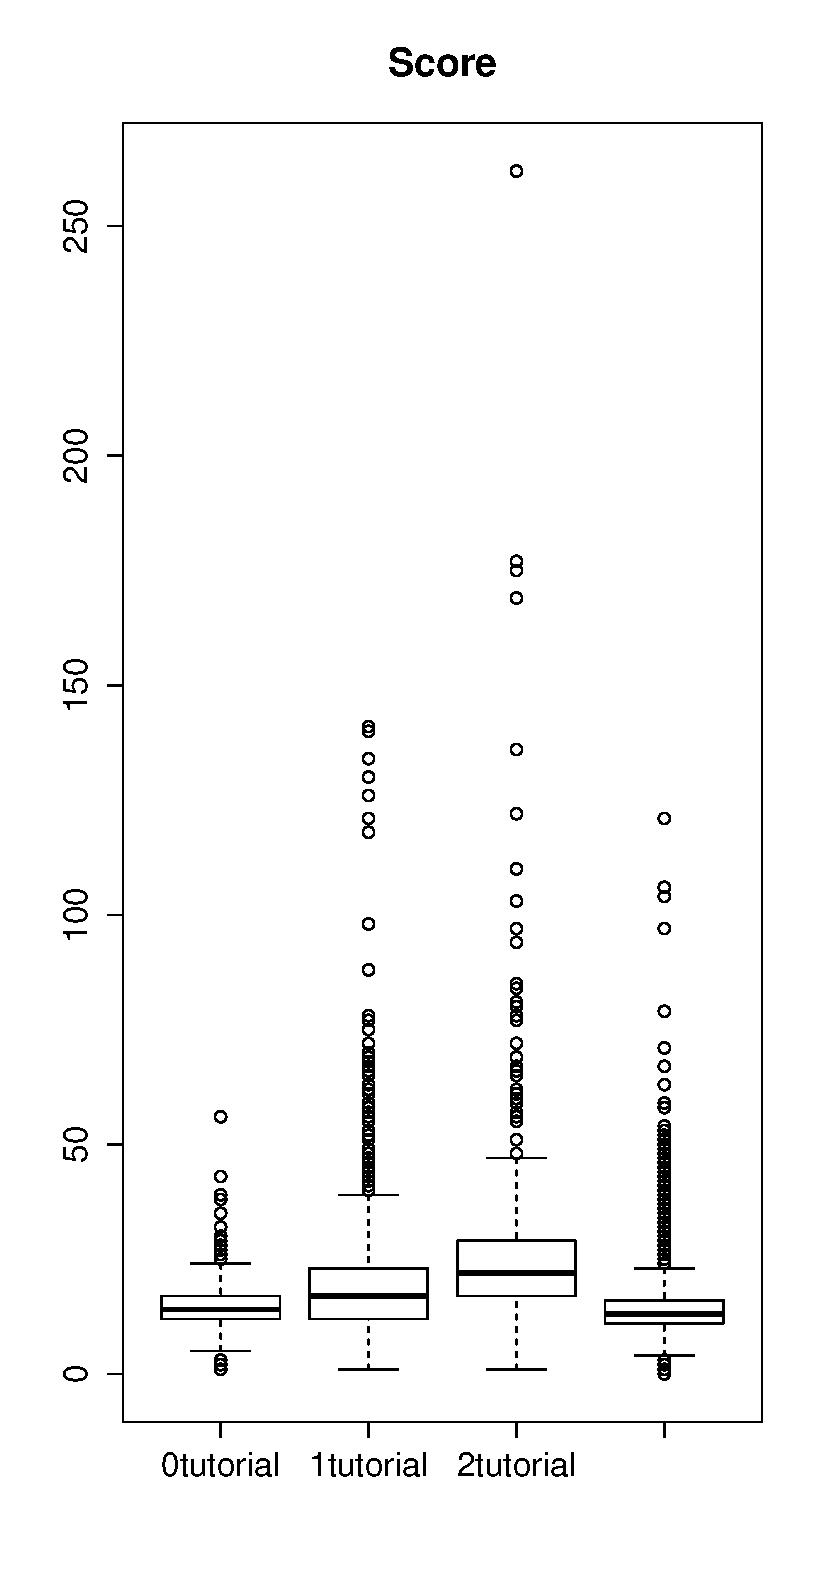
\includegraphics[width=\columnwidth]{figures/preliminary/score_boxplot}

%!TEX root = touchdevelop_tutorials.tex

\subsection{\rqlearning}

We built a linear regression model to identify factors that influenced tutorial completion.



%!TEX root = touchdevelop_tutorials.tex
\section{Conclusion}
The conclusion goes here.


% An example of a floating figure using the graphicx package.
% Note that \label must occur AFTER (or within) \caption.
% For figures, \caption should occur after the \includegraphics.
% Note that IEEEtran v1.7 and later has special internal code that
% is designed to preserve the operation of \label within \caption
% even when the captionsoff option is in effect. However, because
% of issues like this, it may be the safest practice to put all your
% \label just after \caption rather than within \caption{}.
%
% Reminder: the "draftcls" or "draftclsnofoot", not "draft", class
% option should be used if it is desired that the figures are to be
% displayed while in draft mode.
%
%\begin{figure}[!t]
%\centering
%\includegraphics[width=2.5in]{myfigure}
% where an .eps filename suffix will be assumed under latex, 
% and a .pdf suffix will be assumed for pdflatex; or what has been declared
% via \DeclareGraphicsExtensions.
%\caption{Simulation Results}
%\label{fig_sim}
%\end{figure}

% Note that IEEE typically puts floats only at the top, even when this
% results in a large percentage of a column being occupied by floats.


% An example of a double column floating figure using two subfigures.
% (The subfig.sty package must be loaded for this to work.)
% The subfigure \label commands are set within each subfloat command, the
% \label for the overall figure must come after \caption.
% \hfil must be used as a separator to get equal spacing.
% The subfigure.sty package works much the same way, except \subfigure is
% used instead of \subfloat.
%
%\begin{figure*}[!t]
%\centerline{\subfloat[Case I]\includegraphics[width=2.5in]{subfigcase1}%
%\label{fig_first_case}}
%\hfil
%\subfloat[Case II]{\includegraphics[width=2.5in]{subfigcase2}%
%\label{fig_second_case}}}
%\caption{Simulation results}
%\label{fig_sim}
%\end{figure*}
%
% Note that often IEEE papers with subfigures do not employ subfigure
% captions (using the optional argument to \subfloat), but instead will
% reference/describe all of them (a), (b), etc., within the main caption.


% An example of a floating table. Note that, for IEEE style tables, the 
% \caption command should come BEFORE the table. Table text will default to
% \footnotesize as IEEE normally uses this smaller font for tables.
% The \label must come after \caption as always.
%
%\begin{table}[!t]
%% increase table row spacing, adjust to taste
%\renewcommand{\arraystretch}{1.3}
% if using array.sty, it might be a good idea to tweak the value of
% \extrarowheight as needed to properly center the text within the cells
%\caption{An Example of a Table}
%\label{table_example}
%\centering
%% Some packages, such as MDW tools, offer better commands for making tables
%% than the plain LaTeX2e tabular which is used here.
%\begin{tabular}{|c||c|}
%\hline
%One & Two\\
%\hline
%Three & Four\\
%\hline
%\end{tabular}
%\end{table}


% Note that IEEE does not put floats in the very first column - or typically
% anywhere on the first page for that matter. Also, in-text middle ("here")
% positioning is not used. Most IEEE journals/conferences use top floats
% exclusively. Note that, LaTeX2e, unlike IEEE journals/conferences, places
% footnotes above bottom floats. This can be corrected via the \fnbelowfloat
% command of the stfloats package.




% conference papers do not normally have an appendix


% use section* for acknowledgement
\section*{Acknowledgment}


The authors would like to thank...





% trigger a \newpage just before the given reference
% number - used to balance the columns on the last page
% adjust value as needed - may need to be readjusted if
% the document is modified later
%\IEEEtriggeratref{8}
% The "triggered" command can be changed if desired:
%\IEEEtriggercmd{\enlargethispage{-5in}}

% references section

% can use a bibliography generated by BibTeX as a .bbl file
% BibTeX documentation can be easily obtained at:
% http://www.ctan.org/tex-archive/biblio/bibtex/contrib/doc/
% The IEEEtran BibTeX style support page is at:
% http://www.michaelshell.org/tex/ieeetran/bibtex/
\bibliographystyle{IEEEtran}
% argument is your BibTeX string definitions and bibliography database(s)
\bibliography{end_user_programming,stc_model}




% that's all folks
\end{document}


